\chapter{Previous Work}\label{chap:litReview}

Laureti et al. \cite{laureti2006information} introduced iterative filtering as an aggregation method. It set out to appropriate some methods for examining complex networks that had been looked into within the physics community and apply them to scoring systems on the internet. They found that a reciprocal variance method was highly effective at reducing the effects of systemic errors and collusion. They were primarily concerned with the use case of voting on the internet and demonstrated how the reciprocal variance weighting system described in equation \ref{eq:negRecip} would reduce the effectiveness of a cheater the more they cheated, as demonstrated in figure \ref{fig:recipCheating}.

\begin{figure}[H]
    \centering
    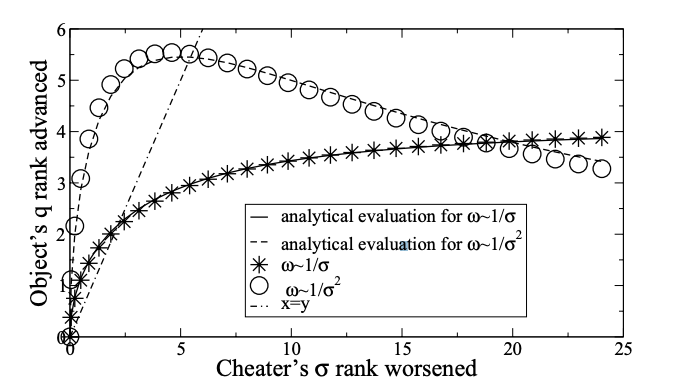
\includegraphics{Figures/recipCheating.png}
    \caption[Relationship between voters accuracy and marginal effect of their vote on an object]{Relationship between voters accuracy and marginal effect of their vote on an object, from \textcite{laureti2006information}.}
    \label{fig:recipCheating}
\end{figure}

De Kerchoove and Van Dooren \cite{de2007iterative} went on to improve applicability of the algorithm by examining a variety of weighting functions, including the affine method defined recursively in equations \ref{eq:affine} and \ref{eq:affineBase}, in order to account for predictable human behaviours, such as clumsiness or dishonesty. They did this by augmenting the MovieLens dataset with a group of random voters and a group that colluded to increase the ratings of a set of movies. Both groups were shown to have significantly reduced trust ratings compared to real voters.
They further examine iterative filtering as it could be a applied to dynamical systems, i.e. one where the set of ratings and raters are non-stationary over time. The examination of such a system is particularly relevant to the topic of this thesis, however they do not examine the case of ratings degradation to preempt changes in quality over time, an issue likely to be critical to this project.  Their experiments validated a slightly modified\footnote{Limiting the number of iterations rather than continuing until convergence was found to provide adequate results while still allowing for rapid updates of ratings.} reciprocal variance method for use within dynamical systems. They also performed a number of experiments to show that IF is very useful for cheater detection. 

\begin{align}
    \tilde{u}^{(n)} &= \sum\limits_{i \in R}\frac{\frac{r_i}{|r_i-\tilde{u}^{(n-1)}|+\epsilon}}{\sum\limits_{j\in R} \frac{1}{|r_j-\tilde{u}^{(n-1)}|+\epsilon}} \label{eq:affine} \\
    \tilde{u}^{(0)} &= \frac{\sum\limits_{i\in R} r_i}{|R|}\label{eq:affineBase}
\end{align}


De Kerchoove and Van Dooren's \cite{de2010iterative} second paper in the area went into great detail regarding the mathematical properties of the various quadratic and affine weighting methods available and demonstrated the validity of all of the methods specified in table \ref{tab:deKerchWeight}. The paper goes on to examine the effects of a very sparse voting matrix, noting that even extreme sparsity does not invalidate any of the ideal properties of the examined algorithms, including robustness against cheating or randomness. Futher, the paper demonstrates the effectiveness of modified techniques, such as specifying various constants (specifically increasing $k$ seen in table \ref{tab:deKerchWeight}), in aggregating such sparse information.

\begin{table}[H]
    \centering
    \begin{tabular}{c c}
    \toprule\toprule
    Weighting System & Formula of Weight \\ \midrule
    Reciprocal Variance & $\frac{1}{\sigma^2}$ \\
    \addlinespace
    Reciprocal Standard Deviation & $\frac{1}{\sigma}$\\
    \addlinespace
    Exponential & $e^{-kd}$ \\
    \addlinespace
    Affine & $1-kd$ \\ \bottomrule
    \end{tabular}
    \caption[Common IF weighting systems]{Common IF weighting systems examined by De Kerchoove and Van Dooren \cite{de2010iterative}, with $d$ refering to absolute distance between a rating and the calculated mean and $k$ being some constant}
    \label{tab:deKerchWeight}
\end{table}

These techniques will likely be very useful when it comes to designing a system that can handle recommendations about small-cap stocks which are typically under-covered by analysts. By ensuring that the method chosen is valid for all securities, the system could be more easily expanded and automated for a larger range of financial products.

Zhou et al. \cite{zhou2011robust} added to the current set of quadratic and affine weighting paradigms by designing a system that used the correlation of a user's rating and an objects rating to enhance it's assignment of weights (seen in equation \ref{eq:qbullshit}). This method was shown to be very effective in aggregating datasets with a high ratio of spammers however did not perform as well as other algorithms in datasets with a lower ratio. Depending on the quantity of analysts with no significant skill this method may be quite useful.


\begin{equation}
    \tau_i = max\left(0, 
    \frac{1}{|j:i\rightarrow j|}
    \sum\limits_{j:i\rightarrow j}
    \left(\frac{r_{i,j} - \bar{r}_i}{\sigma_{r_i}}\right)
    \left(\frac{v_{j} - \bar{v}_{j:i\rightarrow j}}{\sigma_{v_{j:i\rightarrow j}}}\right)
    \right) \label{eq:qbullshit}
\end{equation}

Ignjatovic et al. \cite{ignjatovic2009computing} specifically examined the case of multiple assessors marking assignments and considered specifically the cases that a case of systemic bias as well as providing methods to adjust for issues that are likely to be encountered, such as a small number of markers per assessment, in which case there are suggested parameter modifications. This naturally flows over into the problem at hand where the number and frequency of recommendations is likely to correlate quite strongly with the market cap of the stock and thus a system may need to take issues like this into account when aggregating ratings in order to provide more valid recommendations.

Rezvani et al. \cite{rezvani2018provenance} examined several significant modifications and addons to other methods and looked specifically into provenance, i.e. external factors that could be used to augment trust ratings. Potential factors that might aid in producing more valid results are explored in section \ref{sec:plan}.

The literature in the area has produced multiple techniques that will aid significantly in the development of an algorithm to aggregate financial data. Particularly, approaches for dynamical systems, sparse voting patterns, dealing with collusion and bias, and accounting for provenance are specified and validated. In order to incorporate these techniques, several procedures that aren't investigated by the literature will need to investigated, namely the specific configuration of algorithm to best deal with combination of sparsity, white noise, and systematic bias that occurs in financial data, a trust system that expects, rather than allowing for, changes in the quality of a reviewer, and methods for deriving provenance factors.